% Chaptre 1

\chapter{Outils et technologies utilisés} % Main chapter title

\label{Chaptre3} % For referencing the chapter elsewhere, use \ref{Chapter1} 

Dans cette section je vais présenter les outils et les technologies que j’avais utilisé durant mon stage.

%----------------------------------------------------------------------------------------

% Define some commands to keep the formatting separated from the content 
%\newcommand{\keyword}[1]{\textbf{#1}}
%\newcommand{\tabhead}[1]{\textbf{#1}}
%\newcommand{\code}[1]{\texttt{#1}}
%\newcommand{\file}[1]{\texttt{\bfseries#1}}
%\newcommand{\option}[1]{\texttt{\itshape#1}}
%----------------------------------------------------------------------------------------

\section{Amazon Lambda}
AWS Lambda est un service de calcul Serverless qui vous permet d’exécuter du code sans:
\begin{list}{•}
	\item provisionner ou gérer des serveurs,
	\item créer une logique de dimensionnement de cluster prenant en charge la charge de travail,
	\item  maintenir les intégrations d’événements ou gérer les environnements d’exécution.
\end{list}
Avec Lambda, vous pouvez exécuter du code pour pratiquement n’importe quel type d’application ou service backend , sans aucune tâche administrative. Il suffit de télécharger votre code sous forme de fichier
ZIP ou d’image de conteneur, et Lambda alloue automatiquement et précisément la puissance d’exécution
de calcul et exécute votre code en fonction de la demande ou de l’événement entrant, pour n’importe quelle
échelle de trafic.
Vous pouvez configurer votre code de sorte qu’il se déclenche automatiquement depuis plus de 200 applications SaaS et services AWS, ou l’appeler directement à partir de n’importe quelle application web ou
mobile.
Vous pouvez écrire des fonctions Lambda dans votre langage préféré (Node.js, Python, Go, Java, etc.)
\subsection{Fonctionnement}
Chaque fonction Lambda s'exécute dans son propre conteneur. Lorsqu'une fonction est créée, Lambda l'empaquette dans un nouveau conteneur, puis exécute ce conteneur sur un cluster de machines mutualisées géré par AWS. Avant que les fonctions ne commencent à s'exécuter, le conteneur de chaque fonction se voit allouer la mémoire RAM et la capacité CPU nécessaires. Une fois que les fonctions ont fini de s'exécuter, la RAM allouée au début est multipliée par le temps que la fonction a passé à s'exécuter. Les clients sont ensuite facturés en fonction de la mémoire allouée et de la durée d'exécution de la fonction.
\subsection{Avantages}
\begin{list}{•}
	\item Aucun serveur à gérer:
	AWS Lambda exécute automatiquement votre code, sans que vous ayez à mettre en service ou à gérer des
	serveurs
	\item Dimensionnement continu:
	AWS Lambda dimensionne automatiquement votre application en exécutant le code en réponse à chaque
	déclencheur. Votre code s’exécute en parallèle et traite chaque déclencheur indépendamment. La charge de
	travail est ainsi mise à l’échelle de façon précis
	\item Optimisation des coûts grâce au comptage en millisecondes:
	Avec AWS Lambda, vous ne payez que pour le temps de calcul que vous consommez
	\item Performances constantes à n’importe quelle échelle:
	Avec AWS Lambda, vous pouvez optimiser le temps d’exécution de votre code en choisissant la bonne taille de mémoire pour
	votre fonction
\end{list}

%----------------------------------------------------------------------------------------

\section{Docker}
Docker est un système de containérisation le plus utilisé; qui vous permet de créer, déployer et lancer vos applications en utilisant des conteneurs.
Pour mettre en place ces conteneurs, on crée des images Docker. L’image Docker permet de configurer tout l’environnement dans lequel le conteneur va s'exécuter. 
Pour créer ces images, Docker utilise un fichier spécial appelé Dockerfile, qui grâce à une syntaxe simple et élégante va nous permettre de préparer nos images.
L’image est ensuite construite par le démon Docker via l’utilisation de commandes dans le terminal qui sont regroupées dans ce qu’on appelle un CLI.
Pour gérer l’ensemble des conteneurs d’une application, on utilise Docker Compose.

 \begin{figure}[H]
            \centering
                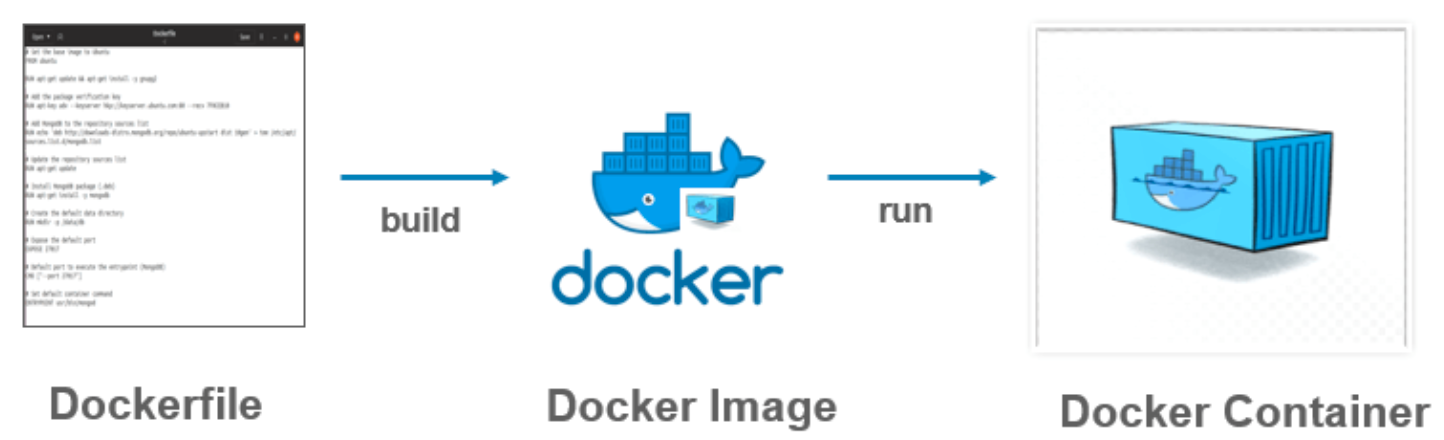
\includegraphics[width=0.8\textwidth]{Figures/dockerfileimagecontainer}
	       \decoRule
		\caption[Docker]{Docker}
	\label{fig:docker}
\end{figure}
Un conteneur est une instance d'une image et une image est obtenue on compilant le fichier Dockerfile.
\subsection{Docker Hub}
Docker Hub est un service fourni par Docker pour rechercher et partager des images de conteneurs avec votre équipe. 
Il s'agit du plus grand référentiel au monde d'images de conteneurs.
Docker Hub fournit les fonctionnalités principales suivantes :
\begin{list}{•}
	\item Repositories: permet le push et le pull des images des conteneurs
	\item Teams and  Organizations: permet de gérer l'accès aux référentiels privés d'images de conteneurs
	\item Docker Official Images: permet de récupéré  et d'utiliser des images de conteneurs de haute qualité fournies par Docker
	\item Builds: permet de créer automatiquement des images de conteneur à partir de GitHub et Bitbucket et de les transférer vers Docker Hub.
\end{list}
Docker fournit un outil  Docker Hub CLI  et une API qui vous permet d'interagir avec Docker Hub.


\section{Amplify}

AWS Amplify est un ensemble d’outils et de services qui peuvent être utilisés ensemble ou un par un, pour:
\begin{list}{•}
\item Authentification: accéder à des workflows prêts à l'emploi pour MFA, authentification unique, mot de passe oublié, etc.
\item Hébergement: déployer des applications Web statiques en quelques clics et facilement gérer le contenu(JavaScript, React, Angular, Flutter,...)
\item Notifications push: gérer facilement les campagnes et envoyer des messages aux utilisateurs via plusieurs canaux, notamment par SMS, e-mail et push.
\item Analytique: suivre les sessions des utilisateurs et créer des rapports sur leur comportement. Configurer des attributs personnalisés et analyser les entonnoirs de conversion.
\end{list}

%link : https://www.bluematador.com/blog/what-is-aws-amplify
%aider les développeurs web mobile et frontal à créer des applications évolutives et intégrales à technologie
%AWS. Avec Amplify, vous pouvez configurer les backends d’application et connecter votre application en
%quelques minutes, déployer des applications Web statiques en quelques clics et facilement gérer le contenu
%des applications en dehors de la console AWS.
%Amplify prend en charge les frameworks Web populaires, tels que JavaScript, React, Angular, Vue, Next.js,
%et les plateformes mobiles, telles qu’Android, iOS, React Native, Ionic, Flutter.
%\subsubsection{Developpement}
 \begin{figure}[H]
            \centering
                \includegraphics[width=0.8\textwidth]{Figures/amplify_dif}
	       \decoRule
		\caption[Exemple d'hébergement d'un site static]{Exemple d'hébergement d'un static}
	\label{fig:amplify}
	\end{figure}
%\subsubsection{}
% \begin{figure}[H]
%            \centering
%              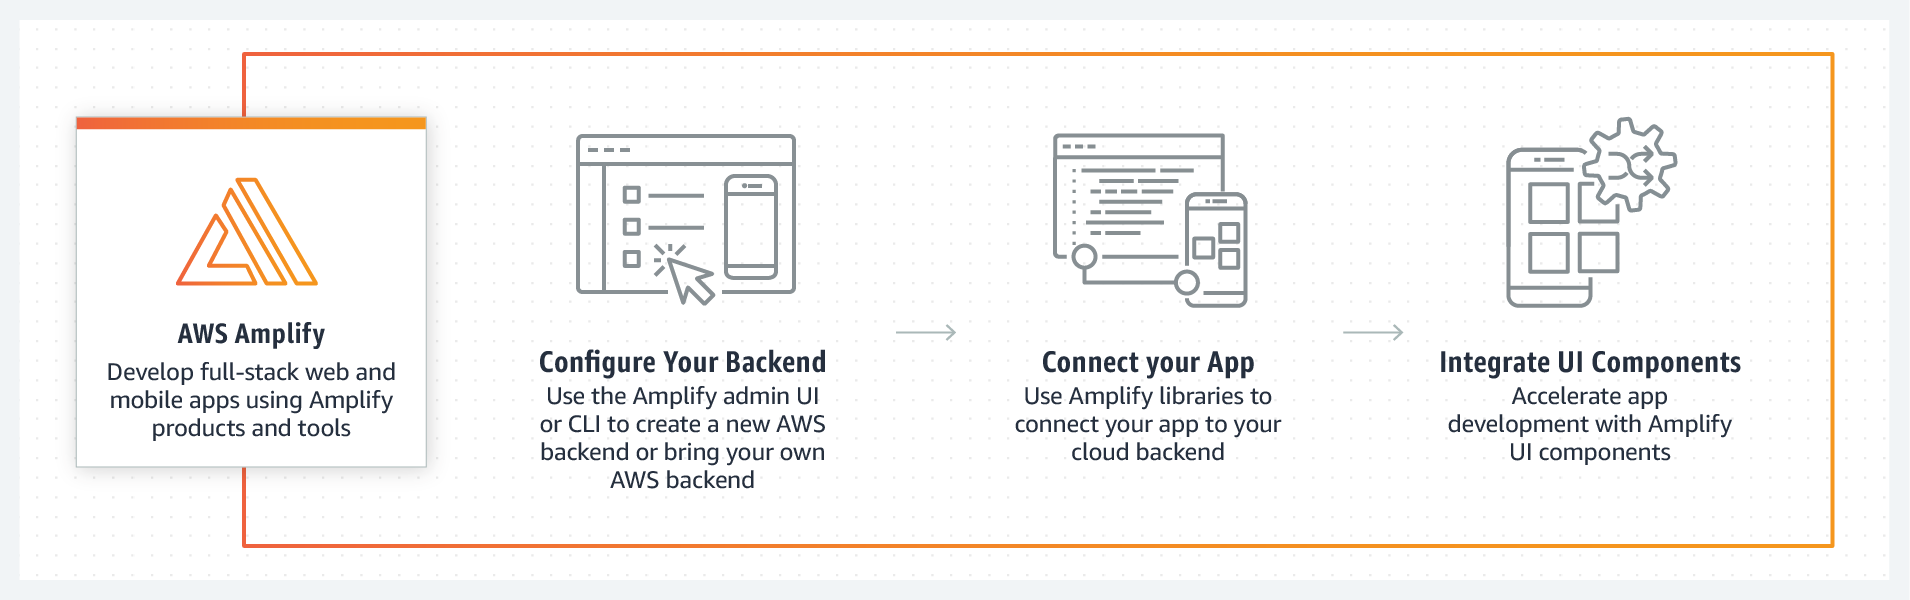
\includegraphics[width=0.8\textwidth]{Figures/amplify-2}
%	       \decoRule
%		\caption[Amplify]{Amplify}
%	\label{fig:amplify}
%	\end{figure}

\section{Amazon Simple Storage Service (Amazon S3)}
Amazon S3 est un stockage d'objets conçu pour stocker et récupérer n'importe quelle quantité de données, n'importe où. Il s'agit d'un service de stockage simple qui offre une durabilité, une disponibilité, des performances, une sécurité, et une scalabilité de pointe pratiquement illimitée à un tarif très bas.
S3 supporte tout type de fichier et peut être utilisé comme repos d'hébergement des sites web statics:
\subsection{Avantages de l'utilisation d'Amazon S3}
Amazon S3 est intentionnellement conçu avec un ensemble de fonctionnalités minimal qui met l'accent sur la simplicité et la robustesse. Voici quelques-uns des avantages de l'utilisation d'Amazon S3 :
\begin{list}{•}
\item \textbf{Création de compartiments:}Créez et nommez un compartiment qui stocke les données. Les compartiments sont les conteneurs fondamentaux d'Amazon S3 pour le stockage de données.
\item \textbf{Stockage de données:}Stockez une quantité infinie de données dans un bucket. Chargez autant d'objets que vous le souhaitez dans un compartiment Amazon S3. Chaque objet peut contenir jusqu'à 5 To de données. Chaque objet est stocké et récupéré à l'aide d'une clé unique attribuée par le développeur.
\item \textbf{Téléchargement de données:}Téléchargez vos données ou permettez à d'autres de le faire. Téléchargez vos données à tout moment ou permettez à d'autres de faire de même.
\item \textbf{Autorisations:}Accordez ou refusez l'accès à d'autres personnes qui souhaitent charger ou télécharger des données dans votre compartiment Amazon S3. Accordez des autorisations de chargement et de téléchargement à trois types d'utilisateurs. Les mécanismes d'authentification peuvent aider à protéger les données contre les accès non autorisés.
\item \textbf{Interfaces standard:}Utilisez des interfaces REST et SOAP basées sur des normes conçues pour fonctionner avec n'importe quelle boîte à outils de développement Internet.
\end{list}


%S3 est un service de stockage d’objet offrant une évolutivité, une disponibilité des données, une sécurité et des performances de pointe. Les clients de toutes tailles et de tous secteurs peuvent ainsi utiliser
%ce service afin de stocker et protéger n’importe quelle quantité de données pour un large éventail de cas
%d’utilisation comme des lacs de données, des sites web, des applications mobiles, la sauvegarde et la restauration, l’archivage, des applications d’entreprise, des appareils IoT et des analyses du Big Data. Amazon
%S3 fournit des fonctions de gestion faciles à utiliser pour vous permettre d’organiser vos données et de
%configurer des contrôles d’accès affinés pour vos exigences métier, d’organisation et de conformité spécifiques. Amazon S3 est conçu pour offrir 99,999999999 \% de durabilité et stocker les données de millions
%d’applications pour des entreprises du monde entier

\section{Aws Aurora}

Amazon Aurora est un moteur de base de données relationnelle qui associe la vitesse et la fiabilité des bases
de données commerciales haut de gamme à la simplicité et la rentabilité des bases de données open source.
Amazon Aurora MySQL offre des performances jusqu’à cinq fois supérieures à celles de MySQL sans
nécessiter de modifications de la plupart des applications MySQL. De la même manière, Amazon Aurora
PostgreSQL offre des performances jusqu’à trois fois supérieures à celles de PostgreSQL. Amazon RDS
gère vos bases de données Amazon Aurora en prenant en charge les tâches chronophages telles que la mise en service, l’application des correctifs, la sauvegarde, la récupération, la détection des pannes, ainsi que
les réparations. Vous payez un forfait mensuel pour chaque instance de base de données Amazon Aurora
utilisée. Aucun coût initial ou engagement à long terme n’est requis.

\subsection{Que signifie « des performances trois fois supérieures à celles de PostgreSQL  et MySQL» }
Amazon Aurora fournit des augmentations significatives des performances de PostgreSQL et  MySQL en intégrant étroitement au moteur de base de données une couche de stockage virtualisée basée sur SSD, conçue principalement pour les charges de travail des bases de données, ce qui permet de réduire les opérations d'écritures dans le système de stockage, minimiser la contention de verrouillage et éliminer les retards créés par les threads de processus de la base de données

\section{Amazon Cognito}
Amazon Cognito permet d’ajouter facilement et rapidement l’inscription et la connexion des utilisateurs ainsi que le contrôle d’accès aux applications Web et mobiles. Amazon Cognito s’adapte à des millions d’utilisateurs et prend en charge la connexion avec les fournisseurs d’identité sociale tels qu’Apple, Facebook, Google et Amazon.\\ Amazon Cognito prend en charge les normes de gestion des identités et des accès, telle que Oauth 2.0.
%, et les fournisseurs d’identité d’entreprise via SAML 2.0 et OpenID Connect

%\subsection{Fonctionnalités}
%\subsubsection{Répertoire d’utilisateurs sécuritaire et se mettant à l’échelle}Les groupes d’utilisateurs d’Amazon Cognito fournissent un répertoire d’utilisateurs sécurisé qui s’étend à
%des centaines de millions d’utilisateurs. En tant que service entièrement géré, les groupes d’utilisateurs sontfaciles à configurer sans avoir à s’inquiéter de la mise en place d’une infrastructure serveur.
%\subsubsection{Fédération d’identité sociale et d’entreprise}
%Avec Amazon Cognito, vos utilisateurs peuvent se connecter via des fournisseurs d’identité sociale tels
%que Apple, Google, Facebook et Amazon.

%\subsubsection{Authentification basée sur les standards}
%Amazon Cognito User Pools est un fournisseur d’identités normalisé et prend en charge les normes degestion des identités et des accès, telle que Oauth 2.0.
%\subsubsection{Sécurité pour vos applications et vos utilisateurs}
%Amazon Cognito prend en charge l’authentification multi-facteurs et le chiffrement des données au repos et
%en transit. Amazon Cognito est éligible HIPAA et conforme aux normes PCI DSS, SOC, ISO/IEC 27001,ISO/IEC 27017, ISO/IEC 27018, et ISO 9001.
%\subsubsection{Contrôle d’accès pour les ressources AWS}Amazon Cognito fournit des solutions pour contrôler l’accès aux ressources AWS à partir de votre application. Vous pouvez définir des rôles et associer des utilisateurs à des rôles différents afin que votre
%application puisse accéder uniquement aux ressources autorisées pour chaque utilisateur. Autre possibilité: vous pouvez également utiliser les attributs des fournisseurs d’identité dans les stratégies d’autorisationAWS Identity and Access Management. Cela vous permettra de contrôler l’accès à des ressources pour lesutilisateurs qui remplissent des conditions d’attributs spécifiques
%\subsubsection{Intégration facile avec votre application}Amazon Cognito fournit des solutions pour contrôler l’accès aux ressources AWS à partir de votre application. Vous pouvez définir des rôles et associer des utilisateurs à des rôles différents afin que votreapplication puisse accéder uniquement aux ressources autorisées pour chaque utilisateur. Autre possibilité: vous pouvez également utiliser les attributs des fournisseurs d’identité dans les stratégies d’autorisationAWS Identity and Access Management. Cela vous permettra de contrôler l’accès à des ressources pour lesutilisateurs qui remplissent des conditions d’attributs spécifiques.


\section{API Gateway}

Amazon API Gateway est un service entièrement opéré, qui permet aux développeurs de créer, publier,
gérer, surveiller et sécuriser facilement des API à n’importe quelle échelle. Les API servent de « porte
d’entrée » pour que les applications puissent accéder aux données, à la logique métier ou aux fonctionnalités de vos services backend. À l’aide d’API Gateway, vous pouvez créer des API RESTful et des API
WebSocket qui permettent de concevoir des applications de communication bidirectionnelle en temps réel.
API Gateway prend en charge les charges de travail conteneurisées et sans serveur, ainsi que les applications
web.\\
API Gateway gère toutes les tâches liées à l’acceptation et au traitement de plusieurs centaines de milliers
d’appels d’API simultanés, notamment la gestion du trafic, la prise en charge de CORS, le contrôle des
autorisations et des accès, la limitation, la surveillance et la gestion de la version de l’API. Aucuns frais
minimum ou coûts initiaux ne s’appliquent à API Gateway. Vous payez pour les appels d’API que vous
recevez et la quantité de données transférées et, avec le modèle de tarification par paliers de l’API Gateway,
vous pouvez réduire vos coûts en fonction de l’utilisation de votre API

 \begin{figure}[H]
            \centering
                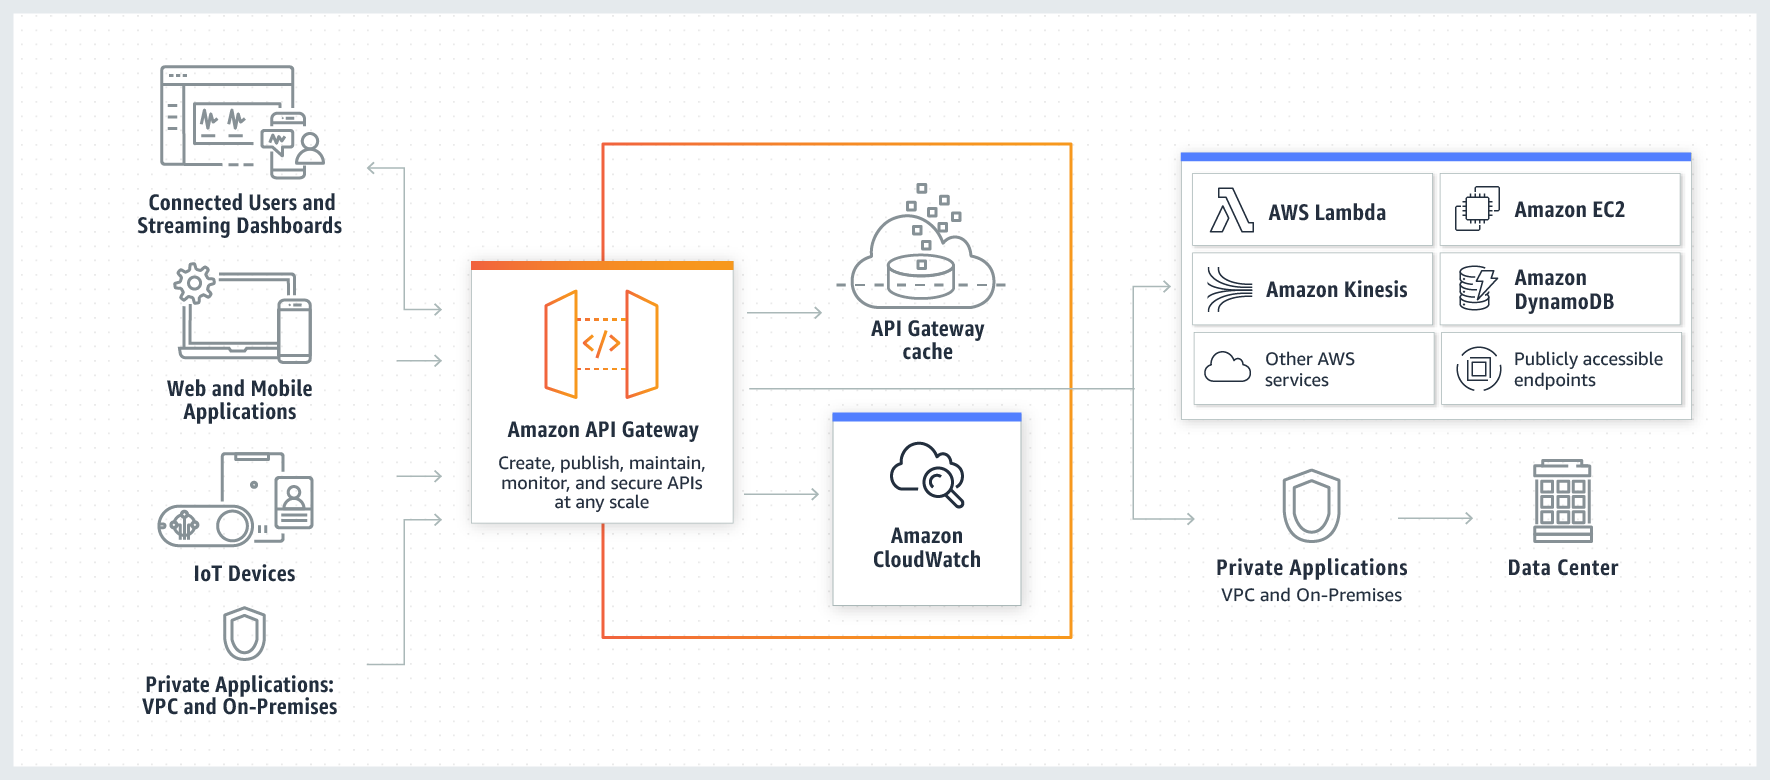
\includegraphics[width=0.8\textwidth]{Figures/apigateway}
	       \decoRule
		\caption[API Gateway]{API Gateway}
	\label{fig:apigateway}
	\end{figure}

%----------------------------------------------------------------------------------------

\section{Amazon Dynamodb}
Amazon DynamoDB est une base de données NoSql de type clé-valeur et de documents, offrant des performances de latence de l’ordre de quelques millisecondes, quelle que soit l’échelle. Il s’agit d’une base
de données multi-région, multi-active et durable entièrement gérée, avec des systèmes intégrés de sécurité,
de sauvegarde, de restauration et de mise en cache en mémoire pour les applications à l’échelle d’Internet.
DynamoDB peut traiter plus de 10 mille milliards de demandes par jour et supporte des pics de 20 millions
de demandes par seconde.\\

La plupart des entreprises du monde qui connaissent la croissance la plus rapide, comme Lyft, Airbnb et
Redfin, ainsi que Samsung, Toyota et Capital One s’appuient sur la mise à l’échelle et les performances de
DynamoDB pour prendre en charge leurs charges de travail stratégiques.
Des centaines de milliers de clients AWS ont choisi DynamoDB comme base de données de clés-valeurs et
de documents pour leurs applications mobiles, Web, de jeux, de technologie publicitaire, IoT, etc. nécessitant un accès à faible latence aux données, quelle que soit l’échelle
\newpage
\section{CloudWatch}
Amazon CloudWatch est un service de surveillance et d'observabilité conçu pour les ingénieurs DevOps, les développeurs, les ingénieurs en fiabilité de sites (SRE) et les responsables informatiques. \\

CloudWatch collecte des données de surveillance et opérationnelles sous forme de journaux, de métriques et d'événements. Ensuite, il les visualise à l'aide de tableaux de bord automatisés pour vous permettre d’avoir une appréciation unifiée de vos ressources, applications et services AWS opérationnels sur AWS et sur site.
 \begin{figure}[H]
            \centering
                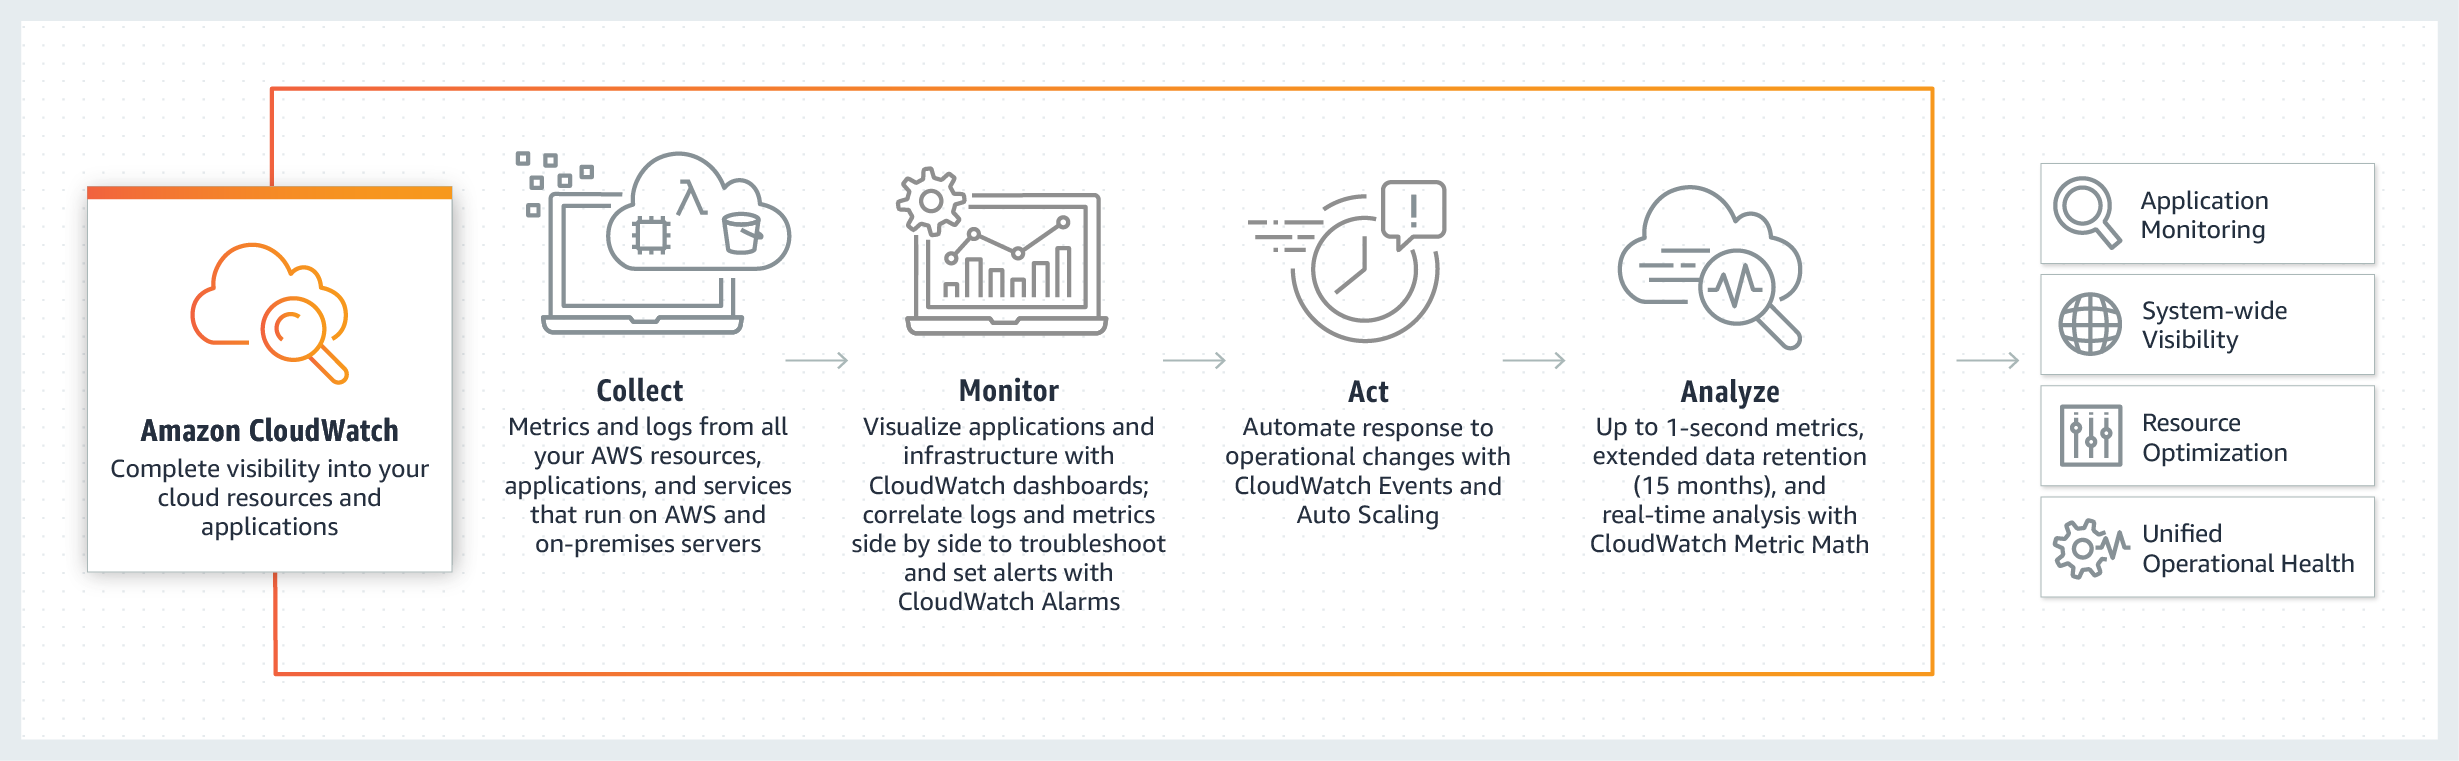
\includegraphics[width=0.8\textwidth]{Figures/cloudwatch}
	       \decoRule
		\caption[CloudWatch]{CloudWatch}
	\label{fig:CloudWatch}
	\end{figure}
\newpage
\section{Reflex}
ReFlex est un système de souscription automatisé modulaire. Il ne s'agit pas d'une application(service web) autonome, elle doit  être intégrée au paysage applicatif du client. Les composants ReFlex requis sont hébergés dans l'environnement du client. Chaque instance de Reflex est fournie avec une base de connaissance paramètrée en fonction des produits d'assurance du client(entreprise d'assurance).
Les principaux modules de Reflex sont:
\begin{list}{•}
\item \textbf{CEP:} Customer Experience Platform
\item
\item \textbf{RAS:} Risk Assessment Service
\item \textbf{DCS:} Document Creation Service 
\end{list}
\subsection{Scénario d'intégration CEP}
En incluant CEP dans le système, toutes les demandes adressées au composant RAS sont filtrées par le backend CEP. Et avant que l'évaluation des risques puisse être lancée, il doit y avoir une toute première étape d'initialisation pour initialiser l'utilisation du CEP. Cette étape comprend l'appel au service d'intégration, qui fait partie du backend CEP, pour créer un jeton Web JSON (JWT) qui sera transmis entre l'interface utilisateur et le backend pour identifier et autoriser l'utilisateur actuel.
 \begin{figure}[H]
            \centering
                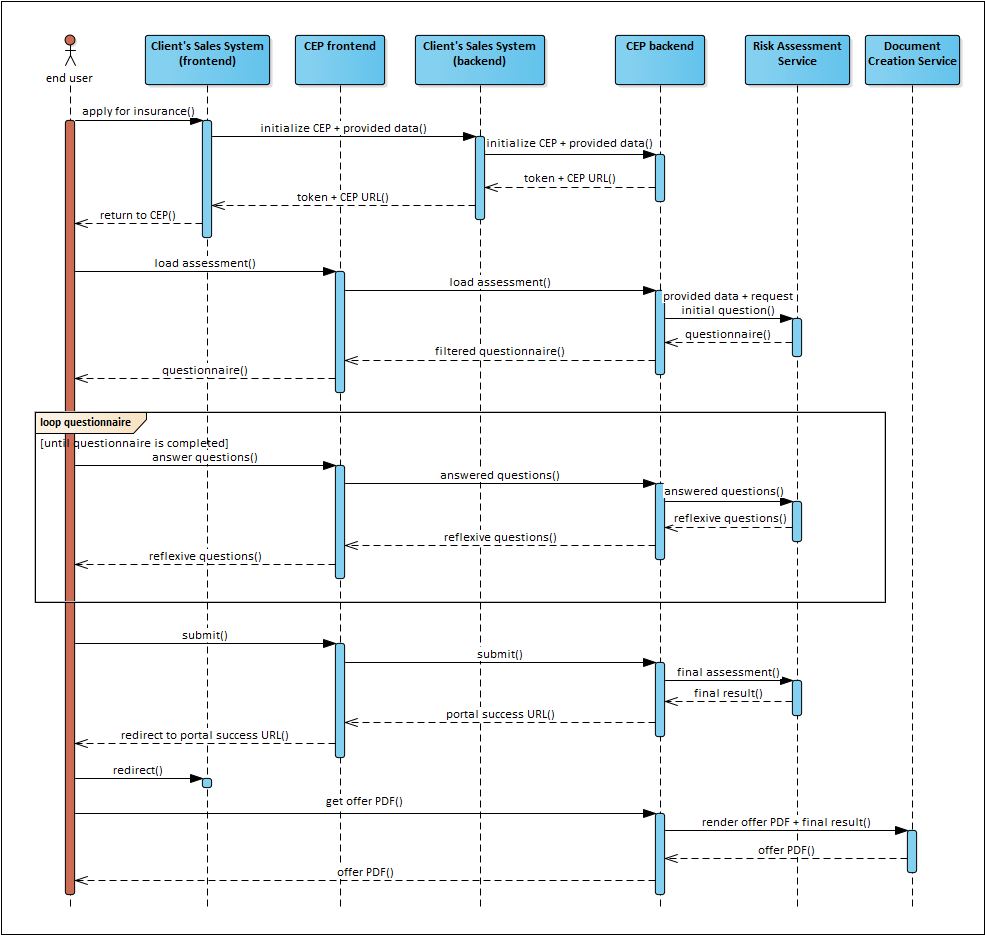
\includegraphics[width=0.8\textwidth]{Figures/cepreflex}
	       \decoRule
		\caption[Scénario d'intégration CEP]{Scénario d'intégration CEP}
\label{fig:Cep}
\end{figure}
